% Préambule
\documentclass[oneside, a5paper, 12pt]{book}
% Configuration des marges
\usepackage[top=0.8in, bottom=0.8in, left=0.8in, right=0.8in]{geometry}

% Personnalisation des titres de section et table des matières
\usepackage{sectsty}
\usepackage{tocloft}
\usepackage[pdftex, pdfauthor={Kevin Delfour}, pdftitle={En Quête d'Expérience : Le chemin du.de la jeune Développeur·euse}, pdfkeywords={développeur, développeuse, expérience, quête, open source}, hidelinks]{hyperref}
\usepackage{chngcntr}
\counterwithout{chapter}{part}

% Cadres, tailles de police et en-têtes/pieds de page personnalisés
\usepackage{framed}
\usepackage{anyfontsize}
\usepackage{fancyhdr}

% Police Garamond et paramètres de langue
\usepackage{ebgaramond}
\usepackage[french]{babel}
\usepackage[T1]{fontenc}
\usepackage{float}

% Couleurs personnalisées et graphiques TikZ
\usepackage[dvipsnames]{xcolor}
\usepackage{tikz}
\usepackage{microtype}
\usepackage{GS1}
\usepackage{qrcode}
\usetikzlibrary{calc}

\usepackage[labelformat=empty]{caption}
\captionsetup{justification=raggedleft, font={tiny, color=gray}, singlelinecheck=false}

% Contenu : texte aléatoire, boucles, images et commandes supplémentaires
\usepackage{lipsum}
\usepackage{pgffor}
\usepackage{graphicx}
\usepackage{etoolbox}

% Configuration de la mise en page
\renewcommand{\familydefault}{\sfdefault}
\setlength{\parskip}{\baselineskip}
\setlength{\parindent}{0pt}

% Configuration de la table des matières
\setcounter{tocdepth}{2}
\renewcommand{\cftpartfont}{\normalfont\bfseries\Large}
\renewcommand{\cftchapfont}{\normalfont\bfseries}
\renewcommand{\cftsecfont}{\normalfont}
\renewcommand{\cftsubsecfont}{\normalfont}
\renewcommand{\cftsubsubsecfont}{\normalfont\small}

% Configuration des en-têtes et pieds de page personnalisés
\pagestyle{fancy}
\fancyhead{}
\fancyhead[LO, L]{ \color{gray}\scriptsize\leftmark}
\fancyfoot{}
\fancyfoot[R]{\scriptsize\thepage}
\renewcommand{\headrulewidth}{0pt}


\newcommand{\customSection}[1]{
	\newpage
	\addcontentsline{toc}{section}{#1}
	\markboth{#1}{#1}
	\section*{#1}
}

\begin{document}
\newpage
% ---- Couverture
\begin{tikzpicture}[overlay,remember picture]
	\node[inner sep=0pt, anchor=south west] at (current page.south west) {
		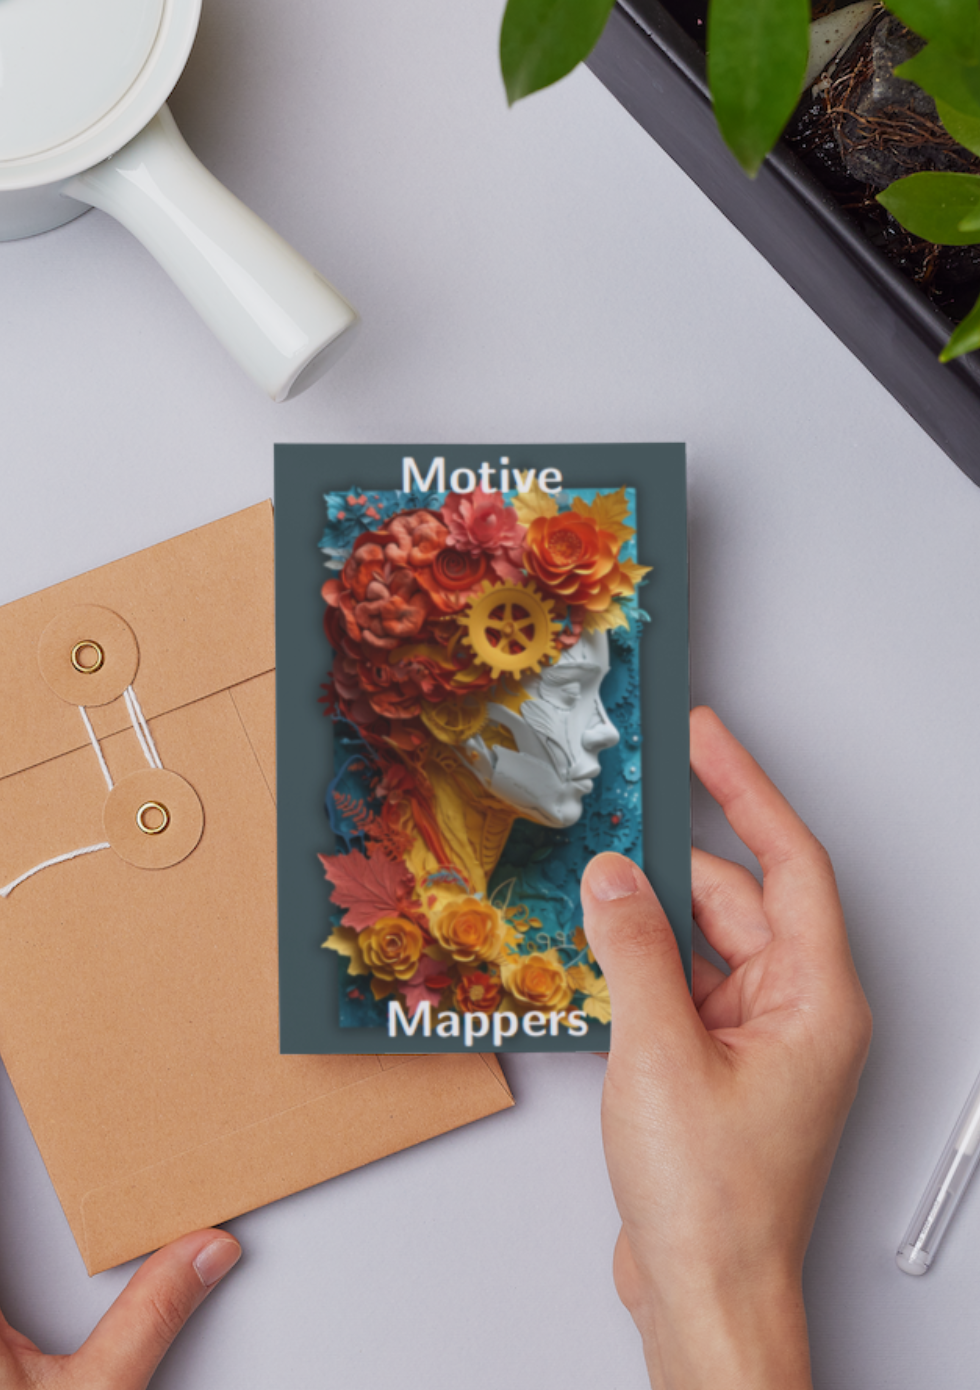
\includegraphics[keepaspectratio, width=\paperwidth]{images/cover-notice.png}
	};

	% Title
	\node[align=center] at ($(current page.center)+(0,-7.5)$)
	{
	{\fontsize{35}{72} \fontfamily{cmr}\selectfont \textcolor{white}{\textbf{Motive Mappers}}}\\[0.5cm]
	{\fontsize{25}{72} \fontfamily{cmr}\selectfont \textcolor{white}{Notice du jeu}}

	};

	% Author
	\node[align=center] at ($(current page.center)+(0,9.2)$)
	{
		{\fontsize{12}{19.2} \textcolor{white}{\selectfont {Max Digital Services Lyon}}}\\[3pt]
	};
\end{tikzpicture}

% ---- Couverture intérieur
\newpage{}
\thispagestyle {empty}
\begin{titlepage}
	\centering
	\vspace*{3cm}
	{\fontsize{35}{72} \fontfamily{cmr}\selectfont \textcolor{black}{\textbf{Motive Mappers}}}\\[0.5cm]
	{\fontsize{25}{72} \fontfamily{cmr}\selectfont \textcolor{black}{Notice du jeu}}\\[0.25cm]
	{\fontsize{12}{19.2} \textcolor{black}{\selectfont {Max Digital Services Lyon}}}\\[3pt]
	\vfill
	\begin{flushleft}
		\textbf{Motive Mappers}, © Max Digital Services Lyon, 2024 \\[0.25cm]
		\textbf{Inspiré du jeu Moving Motivators de Jurgen Apello, Management 3.0 }

		\noindent Ce travail est publié sous la licence Creative Commons Attribution-NonCommercial-ShareAlike 4.0 (BY-NC-SA 4.0). Toutes les parties de ce travail, y compris le texte et les images, sont publiées sous cette licence.
		Certaines images ont été créées en utilisant le service Midjourney par Kévin Delfour, qui détient les droits sur ces images conformément aux termes de service de Midjourney.
		\small{Vous pouvez obtenir une copie de cette licence à l'adresse suivante : \href{http://creativecommons.org/licenses/by-nc-sa/4.0/}{\textcolor{blue}{http://creativecommons.org/licenses/by-nc-sa/4.0/}}}

	\end{flushleft}
\end{titlepage}

% ---- Table des matières
\newpage
\tableofcontents

% ---- Introduction
\customSection{Introduction}

Bienvenue dans l'univers de \textbf{Motive Mappers}, un jeu interactif conçu pour explorer et cartographier les motivations intrinsèques au sein des équipes professionnelles, en particulier dans le domaine de l'IT. Ce jeu offre une approche unique et ludique pour comprendre les facteurs qui motivent individuellement et collectivement, favorisant ainsi un environnement de travail plus harmonieux et productif.

\textit{Motive Mappers} est plus qu'un simple jeu ; c'est un outil de développement personnel et professionnel. En participant à cet atelier, les joueurs auront l'occasion de se plonger dans une introspection significative, de partager leurs expériences et d'apprendre des autres, tout en développant une compréhension plus profonde de ce qui les motive au travail.

L'objectif de ce jeu est de faciliter la communication au sein des équipes, d'augmenter l'engagement et la satisfaction au travail, et de fournir aux leaders et managers des insights précieux pour une gestion plus efficace. Que vous soyez un manager cherchant à renforcer la dynamique de votre équipe, ou un membre d'équipe désireux de mieux comprendre vos propres leviers de motivation, \textbf{Motive Mappers} est l'outil idéal pour vous.

% ---- Contenu du jeu
\customSection{Contenu du Jeu}

\textbf{Motive Mappers} est composé des éléments suivants :

\begin{itemize}
	\item Un ensemble de \textbf{18 cartes de motivation}, chacune représentant une motivation intrinsèque différente. Chaque carte est illustrée par un symbole unique pour faciliter la reconnaissance et la discussion.
	\item Un \textbf{guide de référence rapide} pour chaque carte, décrivant sa signification et son importance dans le contexte professionnel.
	\item Une \textbf{feuilles de score} pour noter les choix et les classements de chaque participant.
\end{itemize}

Voici un résumé des cartes pour "Motive Mappers" avec leurs descriptions :

\begin{itemize}
	\item \textbf{Acceptation} : Besoin de reconnaissance et d'appréciation par les autres.
	\item \textbf{Curiosité} : Désir d'explorer et d'apprendre.
	\item \textbf{Liberté} : Aspiration à l'indépendance et au choix personnel.
	\item \textbf{Honneur} : Engagement envers les valeurs personnelles et l'éthique.
	\item \textbf{Statut} : Quête de reconnaissance sociale ou professionnelle.
	\item \textbf{Maîtrise} : Volonté d'exceller et de développer ses compétences.
	\item \textbf{But} : Désir de poursuivre un travail significatif.
	\item \textbf{Ordre} : Besoin de structure et de clarté.
	\item \textbf{Pouvoir} : Aspiration à influencer et à diriger.
	\item \textbf{Socialisation} : Importance des relations et interactions humaines.
	\item \textbf{Récompense} : Satisfaction de recevoir une compensation juste pour les efforts.
	\item \textbf{Stabilité} : Recherche de sécurité dans la vie professionnelle.
	\item \textbf{Harmonie} : Équilibre entre vie professionnelle et personnelle.
	\item \textbf{Appartenance} : Alignement avec les valeurs et la culture de l'entreprise.
	\item \textbf{Autonomie} : Désir de liberté dans l'organisation du travail.
	\item \textbf{Impact} : Volonté de contribuer positivement à la société.
	\item \textbf{Innovation} : Enthousiasme pour la nouveauté et la technologie.
	\item \textbf{Développement} : Aspiration à la croissance personnelle et professionnelle.
\end{itemize}
Ces cartes représentent un éventail de motivations intrinsèques, facilitant la compréhension et la discussion sur ce qui motive individuellement et collectivement dans un cadre professionnel.

Chaque carte de motivation porte un symbole spécifique, soigneusement choisi pour représenter visuellement le concept de la motivation concernée. Par exemple, la carte \textit{Curiosité} est représentée par une loupe, tandis que la carte \textit{Liberté} montre un oiseau en vol.

% ---- Règles du Jeu
\customSection{Règles du Jeu}

\subsection*{Préparation}
Avant de commencer, chaque participant reçoit un jeu complet de cartes \textbf{Motive Mappers}. Les joueurs sont encouragés à se familiariser avec les cartes et leur signification.

\subsection*{Jeu}
\begin{enumerate}
	\item \textbf{Sélection et Classement} : Chaque participant sélectionne et classe ses 5 principales motivations intrinsèques à partir du jeu de cartes.
	\item \textbf{Discussion} : Les participants partagent et discutent leurs choix avec le groupe, en expliquant pourquoi ils ont choisi et classé leurs cartes de cette manière.
	\item \textbf{Évaluation des Motivations dans le Cadre de Travail Actuel} : Demandez aux participants d'évaluer si les motivations sélectionnées sont présentes dans leur cadre de travail actuel en glissant les cartes vers le haut ou le bas selon leur perception.
	\item \textbf{Réflexion} : Après la discussion et l'évaluation, les participants peuvent choisir de revoir et de réorganiser leurs cartes, basé sur de nouvelles perspectives ou informations.
\end{enumerate}

\subsection*{Objectif}
L'objectif principal de \textbf{Motive Mappers} est de permettre aux participants de mieux comprendre leurs propres motivations et celles des autres, et d'utiliser ces informations pour améliorer la dynamique et l'efficacité de l'équipe.

\subsection*{Durée du Jeu}
Une session typique de \textbf{Motive Mappers} dure environ 45 minutes, mais peut être ajustée selon les besoins du groupe.

% ---- Préparation de la session
\customSection{Préparation de la session}

\subsection*{Matériel Nécessaire}
Assurez-vous d'avoir le matériel suivant avant de commencer la session :
\begin{itemize}
	\item Jeux de cartes \textbf{Motive Mappers}
	\item Feuilles de notes pour les participants
	\item Stylos ou crayons
	\item Espace confortable pour le groupe
\end{itemize}

\subsection*{Configuration de l'Espace}
\begin{itemize}
	\item Organisez les sièges en cercle ou en demi-cercle pour favoriser la discussion de groupe.
	\item Assurez-vous que chaque participant a suffisamment d'espace pour étaler ses cartes.
\end{itemize}

% ---- Déroulement d'une session
\customSection{Déroulement d'une Session}

\subsection*{Introduction (5 minutes)}
\begin{enumerate}
	\item Présentez brièvement le but de l'atelier et son déroulement.
	\item Introduisez le concept des motivations intrinsèques.
\end{enumerate}

\subsection*{Explication des Cartes (5 minutes)}
\begin{enumerate}
	\item Expliquez brièvement chaque carte et son symbolisme.
	\item Répondez aux éventuelles questions.
\end{enumerate}

\subsection*{Sélection et Classement (10 minutes)}
\begin{enumerate}
	\item Les participants choisissent et classent leurs 5 principales motivations intrinsèques.
	\item Encouragez la réflexion personnelle durant cette phase.
\end{enumerate}

\subsection*{Discussion en Groupe (15 minutes)}
\begin{enumerate}
	\item Les participants partagent et discutent leurs choix avec le groupe.
	\item Facilitez une discussion ouverte sur les motivations et leurs impacts.
\end{enumerate}

\subsection*{Évaluation des Motivations dans le Cadre de Travail Actuel (10 minutes)}
\begin{enumerate}
	\item Demandez aux participants d'évaluer si les motivations sélectionnées sont présentes dans leur cadre de travail actuel, en glissant les cartes vers le haut ou le bas.
	\item Encouragez la réflexion sur l'alignement entre leurs motivations et leur environnement professionnel.
\end{enumerate}

\subsection*{Synthèse des Motivations d'Équipe (5 minutes)}
\begin{enumerate}
	\item Les participants identifient les tendances communes et les différences dans les motivations de l'équipe.
	\item Discutez de l'importance de ces découvertes pour le travail en équipe.
\end{enumerate}

\subsection*{Conclusion et Réflexion Finale (2 minutes)}
\begin{enumerate}
	\item Récapitulatif des points clés et des tendances observées.
	\item Session de questions/réponses pour clarifier ou approfondir certains aspects.
\end{enumerate}

% ---- Utilisation en Contexte Professionnel
\customSection{Utilisation en Contexte Professionnel}

\textbf{Motive Mappers} est particulièrement efficace dans les environnements professionnels pour les raisons suivantes :

\begin{itemize}
	\item \textbf{Renforcement de l'équipe :} Le jeu permet aux membres de l'équipe de comprendre et d'apprécier les motivations diverses de chacun, renforçant ainsi la cohésion et la collaboration.
	\item \textbf{Leadership éclairé :} Les managers et leaders peuvent utiliser les insights recueillis pour mieux aligner les tâches et les responsabilités avec les motivations individuelles, améliorant ainsi l'engagement et la productivité.
	\item \textbf{Développement personnel :} Chaque participant gagne en autoconnaissance, un atout précieux pour la croissance personnelle et professionnelle.
\end{itemize}

\subsection*{Conseils pour les Managers}
Les managers peuvent tirer parti de \textbf{Motive Mappers} en :

\begin{enumerate}
	\item Encourageant une participation active et honnête pendant le jeu.
	\item Utilisant les résultats pour discuter des objectifs de carrière et des aspirations des membres de l'équipe.
	\item Intégrant les découvertes dans la planification des projets et la distribution des tâches.
\end{enumerate}

% ---- Conseils pour une session réussie
\customSection{Conseils pour une session réussie}

Pour maximiser l'efficacité de \textbf{Motive Mappers}, gardez à l'esprit les points suivants :

\begin{enumerate}
	\item \textbf{Créer un Environnement Sûr :} Assurez-vous que l'atelier se déroule dans un espace où les participants se sentent à l'aise de partager et d'explorer.
	\item \textbf{Faciliter Activement :} Guidez la discussion et l'interaction pour assurer que tous les participants sont engagés et entendus.
	\item \textbf{Encourager l'Honnêteté :} Motivez les participants à être authentiques dans leurs choix et leurs discussions pour des résultats significatifs.
	\item \textbf{Suivi Post-Atelier :} Proposez des actions ou des discussions de suivi pour intégrer les enseignements de l'atelier dans la pratique professionnelle.
\end{enumerate}

% ---- Conclusion
\customSection{Conclusion}

Nous espérons que \textbf{Motive Mappers} vous offrira une expérience enrichissante, vous aidant à découvrir et à naviguer dans le paysage complexe des motivations intrinsèques. Que ce jeu serve de pont entre la compréhension personnelle et l'efficacité professionnelle, et qu'il inspire une dynamique de travail plus positive et productive.

% ---- FAQ
\customSection{FAQ}

\textbf{Foire aux Questions} :

\begin{itemize}
	\item \textit{Que faire si un participant a du mal à choisir ses motivations ?} \\
	      Encouragez une réflexion ouverte et assurez aux participants qu'il n'y a pas de réponse "correcte" ou "fausse".

	\item \textit{Peut-on utiliser le jeu avec de grandes équipes ?} \\
	      Oui, le jeu peut être adapté à des groupes de différentes tailles en organisant des discussions en sous-groupes.

	\item \textit{Comment intégrer les résultats de l'atelier dans la pratique quotidienne ?} \\
	      Les managers peuvent utiliser les résultats pour informer les décisions de gestion, tandis que les individus peuvent les utiliser pour l'auto-réflexion et le développement personnel.
\end{itemize}

% ---- Contact & support
\customSection{Contact et Support}

Pour toute question supplémentaire, assistance ou commentaires sur \textbf{Motive Mappers}, n'hésitez pas à nous contacter :

\begin{itemize}
	\item \textbf{Email :} Contact@maxds.fr
	\item \textbf{Téléphone :} 06.30.05.48.09
	\item \textbf{Site Web :} https://maxds.fr
\end{itemize}

Votre feedback est essentiel pour nous aider à améliorer constamment ce jeu et le rendre aussi utile et agréable que possible pour tous les participants.

% ---- Licence
\customSection{Licence}
Motive Mappers © 2024 est sous licence Attribution-NonCommercial-ShareAlike 4.0 International\\

Vous êtes autorisé à :
\begin{itemize}
	\item \textbf{Partager} — copier, distribuer et communiquer le matériel par tous moyens et sous tous formats
	\item \textbf{Adapter} — remixer, transformer et créer à partir du matériel\\
\end{itemize}

Selon les conditions suivantes :
\begin{itemize}
	\item \textbf{Attribution}  — Vous devez créditer l'Œuvre, intégrer un lien vers la licence et indiquer si des modifications ont été effectuées à l'Oeuvre. Vous devez indiquer ces informations par tous les moyens raisonnables, sans toutefois suggérer que l'Offrant vous soutient ou soutient la façon dont vous avez utilisé son Oeuvre.
	\item \textbf{Pas d’Utilisation Commerciale}  — Vous n'êtes pas autorisé à faire un usage commercial de cette Oeuvre, tout ou partie du matériel la composant.
	\item \textbf{Partage dans les Mêmes Conditions} — Dans le cas où vous effectuez un remix, que vous transformez, ou créez à partir du matériel composant l'Oeuvre originale, vous devez diffuser l'Oeuvre modifiée dans les même conditions, c'est à dire avec la même licence avec laquelle l'Oeuvre originale a été diffusée.
	\item \textbf{Pas de restrictions complémentaires}  — Vous n'êtes pas autorisé à appliquer des conditions légales ou des mesures techniques qui restreindraient légalement autrui à utiliser l'Oeuvre dans les conditions décrites par la licence.
\end{itemize}

\end{document}
